\begin{surferPage}[칠각형 대칭]{칠각형 대칭을 갖는 $7$차식}
    이 별처럼 생긴 곡면은 $7$차 곡면입니다. 꽤 최근까지 이 곡면이 갖는 $84$개의 특이점은 $7$차식이 가질 수 있는 특이점의 최대 개수였습니다. $2004$년에 들어서야 Oliver labs가 세계기록을 $99$개까지 늘려놨습니다.
  
  
오른쪽 그림에서 보여지는 $3$개의 층은 Chmutov의 $8$차식처럼 체비셰프 다항식을 사용하였기 때문에 만들어집니다. 사실 이 별모양의 곡면은 Chmutov 타입 곡면에서 변형된 것입니다. 평면 곡선 $T_d(x)+T_d(y)$ 가 단지 정칠각형 $S_7(x,y)$ 으로 바뀌었을 뿐이죠. 
   
   \[S_7(x,y) + \lambda \cdot T_d(z) = 0,\]
    여기서 $\lambda\in\RR$. 
    \vspace*{-0.3em}
    \begin{center}
      \begin{tabular}{c@{\qquad}c}
        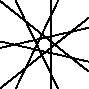
\includegraphics[height=1.5cm]{./../../common/images/labsseptic1.pdf}
        &
        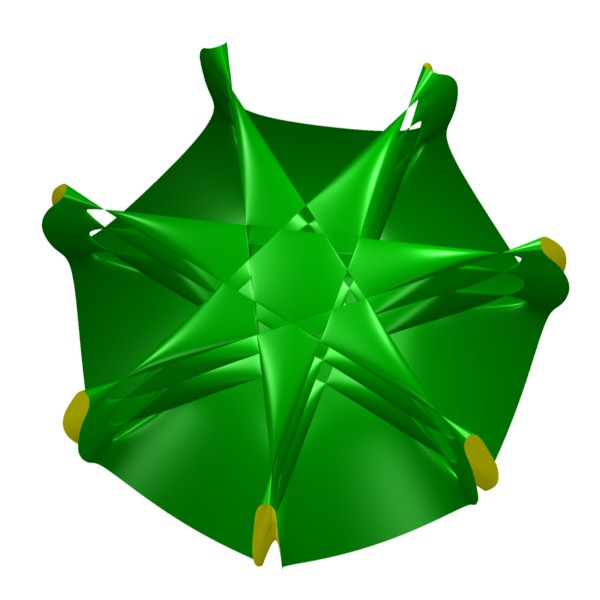
\includegraphics[height=1.5cm]{./../../common/images/septic_7eck_von_oben}
      \end{tabular}
    \end{center}
    \vspace*{-0.3em}   
Chmutov 타입으로부터 변형은 Duco van Straten에 의해 제안되었습니다.
\end{surferPage}
